%Praca inżynierska (c) Kamil Strzempowicz
\documentclass[twoside]{kInzynierka}
%\documentclass[11pt,a4paper]{article}
\usepackage{polski}
%\usepackage[polish]{babel}
\usepackage[utf8]{inputenc}
\usepackage{mathtools}
\usepackage{color}
\usepackage{graphicx}
\usepackage{transparent}
\usepackage{lscape}
\usepackage[section]{placeins}

%hyperref musi być ostatnie
\usepackage[hidelinks]{hyperref}

%%%%%%%%%%%%%%%%%%%%%%%%%%
%%% Przełączniki stylu %%%
%%%%%%%%%%%%%%%%%%%%%%%%%%

\mathtoolsset{showonlyrefs}
\sectionWzory  
%\drukJednostronny
\literowaNumeracjaDodatkow %% w³¹czy numeracjê dodatków literami
%\bezWyjasnien

%%%%%%%%%%%%%%%%%%%%%%%
%%% Podstawowe info %%%
%%%%%%%%%%%%%%%%%%%%%%%

\title{Strategia Just in Time w systemach produkcyjnych\\ - analiza struktury gniazdowej dla heurystyk FIFO i LIFO.}
\promotor{dr inż. Waldemar Grzechca}
\autor{Kamil Strzempowicz}{100}{Napisanie całej pracy}
%% dedykacja mile widziana
\dedykacja{Rodzicom\\bez Was nie udałoby mi się}

%%%%%%%%%%%%%%%%%%%%%%%%%%%%%%%%%
%%% początek właściwej treści %%%
%%%%%%%%%%%%%%%%%%%%%%%%%%%%%%%%%

\begin{document}
\section        {Wstęp}
Celem tej pracy jest przedstawienie strategii Just in Time dla szeregowania zadań w systemach produkcyjnych o strukturze gniazdowej. Szeregowanie przeprowadzono na podstawie heurystyk First In First Out i Last In First Out. Na potrzeby tej pracy powstał program \emph{kSzereg} szeregujący zadania według heurystyk FIFO i LIFO, oraz obliczający wyznaczniki jakosci uszeregowania w kontekście strategii JIT.

System produkcyjny jest to celowo zaprojektowany i zorganizowany układ materialny, energetyczny i informacyjny eksploatowany przez człowieka i służący produkowaniu określonych produktów (wyrobów lub usług) w celu zaspokajania różnorodnych potrzeb konsumentów. \cite{pastuszak}
Systemy produkcyjne można podzielić ze względu na strukturę na:
\begin{itemize}
\item Systemy gniazdowe - zwykle wykorzystywane do pojedyńczych zamówień, bądź krótkich serii. Takie systemy zwykle zmieniają swoje zastosowanie po zakończeniu każdego zlecenia. Zlecenie składa się ze skończonej liczby zadań, a każde z nich wymaga przeprowadzenia zestawu operacji na maszynach w ustalonym porządku, innym dla każdego zadania.
\item System przepływowy - Kierunek przepływu wszystkich zleceń przez maszyny jest ten sam. Dla idealnego systemu przepływowego liczba zadań jest równa liczbie maszyn dla każdego zlecenia. \cite{grzechca}
\item Pojedyńcza maszyna - system składający się z jednej tylko maszyny. Zakłada się, że procesy wytwarzania produktów są jednostadialne, a zlecenia jednostkowe. Stąd zlecenia są tożsame z zadaniami, przy czym nie istnieją ograniczenia kolejnościowe. \cite{grzechca}
\item Maszyny równoległe - system składający się z m identycznych maszyn. Podobnie jak w problemie jednomaszynowym zakłada się, że procesy wytwarzania produktów są jednostadialne, a zlecenia jednostkowe. Stąd, podobnie jak tam, zlecenia są tożsame z zadaniami, przy czym nie istnieją ograniczenia kolejnościowe. \cite{grzechca}
\item Linia montażowa -  zespół stanowisk roboczych (maszynowych, ręcznych lub mieszanych) ugrupowanych według kolejności operacji procesu technologicznego. \cite{wiki}
\end{itemize}

Szeregowanie może zostać zdefiniowne jako przydział zasobów w czasie do zadań w celu optymalizacji kryterium. Z punktu widzenia szeregowania w systemach wytwarzania zasoby często są nazywane maszynami, natomiast jako kryterium optymalności uszeregowania często przyjmowany jest czas potrzebny do zakończenia wszystkich zadań, czy maksymalne spóźnienie zadania. \cite{antColony} 

Problem szeregowania zadań w systmie wytwarzania gniazdowego (skr. JSSP) jest uważany za silnie NP-trudny, czyli co najmniej tak trudny jak każdy problem klasy NP (nondeterministic polynomial), a często trudniejszy. W związku z tym często nie opłaca się tracić czasu i zasobów na poszukiwanie optymalnego rozwiązania JSSP, przyjmuje się natomiast rozwiązanie dopuszczalne uzyskiwane na podstwie przyjętej heurystyki. 
 

\section        [Metody szeregowania zadań \ldots]
		        {Metody szeregowania zadań \newline w systemach wytwarzania gniazdowego}

\subsection     {Metody heurystyczne}
Metody heurystyczne pozwalają na stosunkowo szybkie i łatwe znalezienie dopuszczalnego rozwiązania. Zwykle jednak nie jest to rozwiązanie optymalne, lecz niejednokrotnie bardziej opłacalne jest wdrożenie takiego rozwiązania, niż żmudne poszukiwanie rozwiązania optymalnego, ze względu na czas i zasoby wymagane do jego odnalezienia. W szczególności w sytuacji awaryjnej, gdy nie ma czasu na wykorzystanie bardziej zaawansowanych metod. Metody te zwykle polegają na nadawaniu priorytetu, na podstawie danych zlecenia i chwili czasu, zadaniom w momencie wystąpienia konflktu. 

Konflikt jest to sytuacja gdy w tym samym momencie na dany wolny zasób (maszynę) czeka więcej niż jedno zadanie. Trzeba wtedy zdecydować które z zadań zostanie obsłużone jako pirwsze. 

Najpopularniejsze heurystyki:
\begin{itemize}
\item First In First Out - 
\item Last In First Out - 
\item Earliest Due Date - 
\item Least Work Remaining - 
\item Shortest Procesing Time - 
\item Longest Procesing Time - 
\item Slack Time - 
\item Random - 
\end{itemize}
\subsection     {Inne metody}
\begin{itemize}
\item Algorytmy genetyczne - 
\item Metoda ścieżki krytycznej - 

\end{itemize}

%\newlineTekst
%\newlineSpis
\section        [Heurystyki LIFO i FIFO \ldots]
                {Heurystyki LIFO i FIFO w JSSP \newline - przykłady obliczeniowe}

\subsection     {Różne rozwiązania}
\subsubsection  {FIFO}

\subsubsection  {LIFO}

\subsection     {Identyczne rozwiązania}
\subsubsection  {FIFO}

\subsubsection  {LIFO}

       
\section        {Program kSzereg}
\subsection     {Front-end}
Program kSzereg został wykonany na potrzeby tej pracy dyplomowej.\\

\begin{figure}[htb]
    \centering
    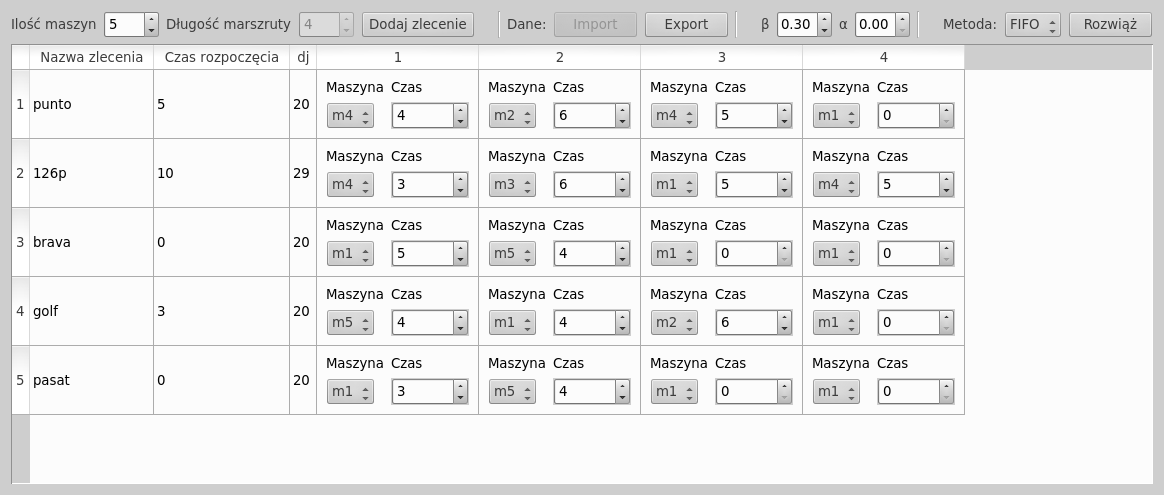
\includegraphics[width=\textwidth, keepaspectratio=true]{./obrazki/main}
    \caption{Główne okno programu}
\end{figure}

\begin{figure}[htb]
    \centering
    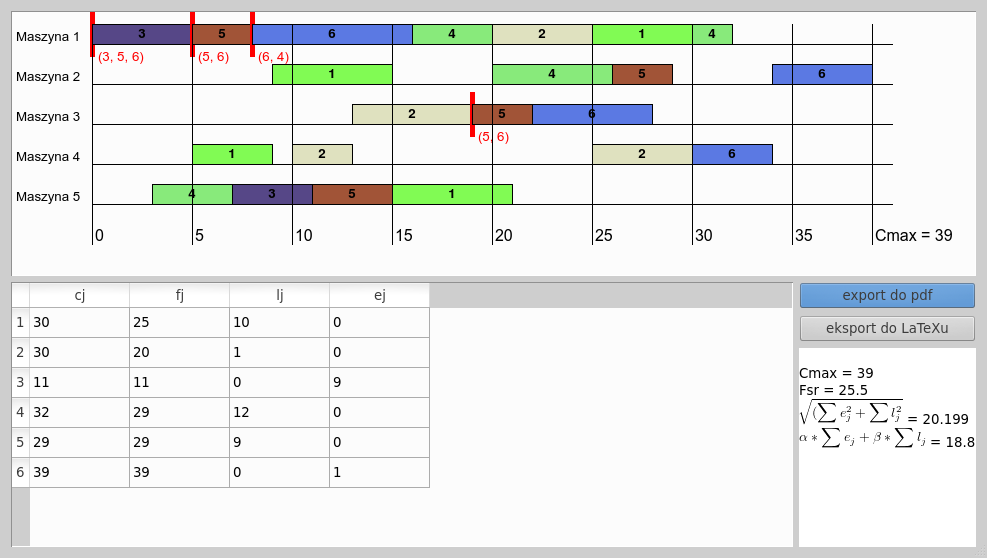
\includegraphics[width=\textwidth, keepaspectratio=true]{./obrazki/wykres}
    \caption{Prezentacja wyznaczonego uszeregowania}
\end{figure}

\begin{figure}[htb]
    \centering
    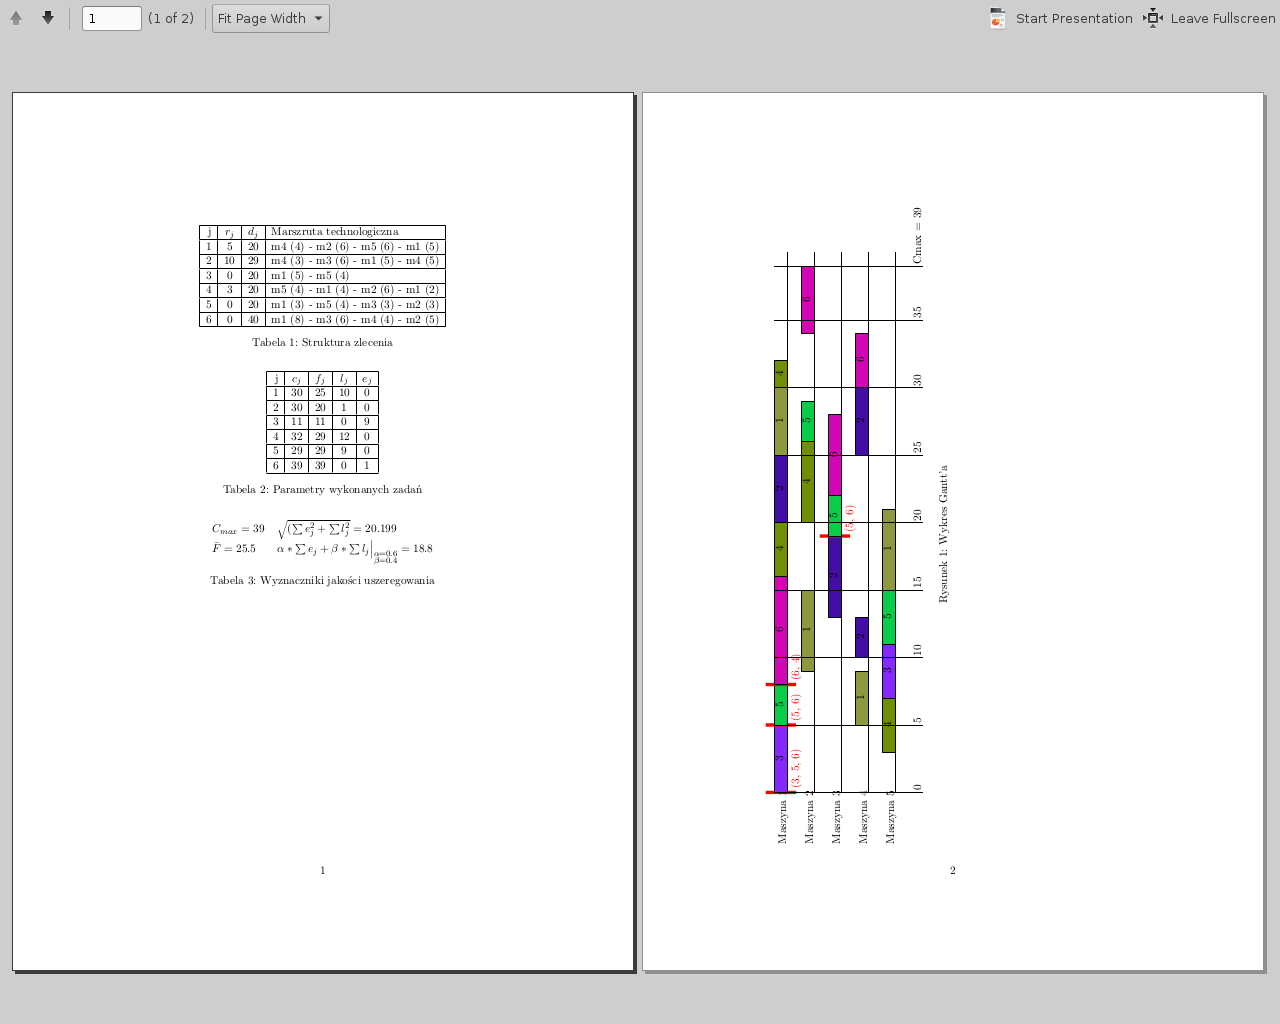
\includegraphics[width=\textwidth, keepaspectratio=true]{./obrazki/pdf}
    \caption{Wyeksportowany plik .pdf}
\end{figure}

\subsection     {Back-end}
  Cały kod źródłowy znajduje się na załączonej płycie cd-rom. \\
Natomiast istotne metody  zosstały przytoczone w dodtku Program \\     
\section        [Przykładowe problemy \ldots]
                {Przykładowe problemy \newline rozwiązane przy pomocy programu kSzereg}
       
\subsection     {Probelm 1}
\subsubsection  {FIFO}
\input {zad1_FIFO.tex}
\subsubsection  {LIFO}
\input{ zad1_LIFO.tex}

\newpage
\subsection     {Problem 2}
\subsubsection  {FIFO}
\input {zad2_FIFO.tex}
\subsubsection  {LIFO}
\input {zad2_LIFO.tex}

\newpage
\subsection     {Problem 3}
\subsubsection  {FIFO}
\input {zad3_FIFO.tex}
\subsubsection  {LIFO}
\input {zad3_LIFO.tex}

\newpage
\subsection     {Problem 3}
\subsubsection  {FIFO}
\input {zad4_FIFO.tex}
\subsubsection  {LIFO}
\input {zad4_LIFO.tex}

\section        {Wnioski}

%\dodatkowo{Programy}
%tu programy
%\begin{verbatim}
%#include <stdio.h>
%int main()
%{
%   printf("Hello world\n");
%}
%\end{verbatim}              
   
\begin{thebibliography}{99}

\bibitem{pastuszak} 
Zarządzanie logistyczne Podstawowe definicje \\
dr Zbigniew Pastuszak

\bibitem{grzechca}
Wykłady z przedmiotu Zautomatyzowane Systemy Wytwarzania\\
dr inż. Waldemar Grzechca na podstawie materiałów prof. dr hab. inż. Mirosława Zaborowskiego \\
Źródło: \url{http://platforma.polsl.pl/rau1} [dostęp:~20.12.12]
\bibitem{wiki}
Linia produkcyjna \\
Źródło: \url{http://pl.wikipedia.org/wiki/Linia_produkcyjna} [dostęp:~20.12.12]

\bibitem{antColony}
    Ant Colony Algorithm for Just-in-Time Job Shop Scheduling with Transportation Times and Multirobots \\
    Fatima El Khoukhi, Tarik Lamoudan, Jaouad Boukachour, Ahmed El Hilali Alaoui




\end{thebibliography}
\end{document}        
